\chapter{Realization}\label{sec:realization}

The realization of the project can be separated into three distinct parts: \textbf{creating wall model}, \textbf{creating hold models} and the \textbf{editor implementation}.
Each of the respective parts are open-source projects on GitHub, licensed under GPLv3:
\begin{itemize}
	\item \raisebox{-0.08em}{\includesvg[height=0.85 \baselineskip]{images/clis.svg}} -- the climber's scanner \footnote{\url{https://github.com/Climber-Apps/Clis}}
	\item \raisebox{-0.08em}{\includesvg[height=0.85 \baselineskip]{images/cled.svg}} -- the climber's editor \footnote{\url{https://github.com/Climber-Apps/Cled}}
\end{itemize}

TODO: discuss other photogrammetry softwares

\section{Creating wall model}
The wall model (figure \ref{fig:model}) has been created semi-automatically.
First, a set of 188 images was used by the Agisoft Metashape software to create a reference model.

While there are other suitable photogrammetry programs such as Meshroom (free), 3DF Zephyr (commercial) and COLMAP (free)

This model was then manually edited in Blender 3D to remove possible modelling errors.
Since the wall consists only of straight segments connected together, this can be done relatively easily.
After manual changes, the resulting model was reimported to Metashape to generate the texture from the photos.

\begin{figure}[H]
	\centering
	\includegraphics[width=\columnwidth]{images/wall/image.png}
	\caption{The model of the Smíchoff wall, created using Metashape and Blender.}
	\label{fig:model}
\end{figure}


\section{Creating hold models}
Since a regular climbing wall contains hundreds or even thousands of holds of varying sizes, it would be infeasible to model each of them manually.
It is important to automate as many steps as possible so that the amount of manual work done is minimized.

This has been accomplished using a turntable-based workflow, upon which the holds are placed and scanned.
The turntable turns the hold around for a stationary camera to take photos, which are then fed into the Agisoft Metashape protogrammetry software (+ Blender for post-processing) to generate the model.

The resulting workflow can process a single hold in $40$ seconds of scanning (taking $12$ photos and varying depending on the lighting conditions) and additional $4$ minutes of processing.

\subsection{Turntable design}
A three stepper-motor turntable has been developed and 3D printed using the Fusion 360 CAD software and an Ender Pro 5 3D printer (figure \ref{fig:turntable}).
An Arduino board and A4988 motor controllers are used for fine motor control (figure \ref{fig:wiring}).
The communication with the Arduino is implemented via the serial port.

\begin{figure}
	\centering
	\includesvg[width=\columnwidth]{images/wiring.svg}
	\caption{The wiring diagram of the turntable, created using Fritzing.}
	\label{fig:wiring}
\end{figure}

To minimize the amount of friction, the only points of contact between the top and bottom part are 7 bearings (6 placed in a circular pattern and 1 directly in the middle).
Additionally, gears mounted to the motors turn the top of the turntable, achieving a 90:12 reduction.
This allows the turntable to handle objects of weight up to TODO (heavier objects have to be turned manually).

\begin{figure}
	% opravdu doufám, že tenhle kód nikdo číst nebude lmao
	\centering
	\subfloat[\centering Top part.]{{\includegraphics[height=3.6cm]{images/turntable/top.png} }}%
	\hfill
	\subfloat[\centering Base part (side).]{{\includegraphics[height=3.6cm]{images/turntable/side.png} }}%
	\hfill
	\subfloat[\centering Base part (top).]{{\includegraphics[height=3.6cm]{images/turntable/bottom.png} }}%
	\\
	\qquad
	\qquad
	\subfloat[\centering Motor mount.]{{\includegraphics[height=2.6cm]{images/turntable/mount.png} }}%
	\hfill
	\subfloat[\centering Motor gear (side).]{{\includegraphics[height=2.6cm]{images/turntable/gear-side.png} }}%
	\hfill
	\subfloat[\centering Motor gear (top).]{{\includegraphics[height=2.6cm]{images/turntable/gear-top.png} }}%
	\qquad
	\qquad
	\quad
	\qquad
	\caption{Parts of the model of the turntable, created using Fusion360.}%
	\label{fig:turntable}
\end{figure}

The top area is connected to a plexiglass with a marked center and 4 markers.

\subsection{Environment setup}
Two LED lights, mounted on adjustable stands and covered with baking paper (for light diffusion) were used to achieve good lighting conditions.
A large black cloth was used as a background around the turntable to minimize the number of unwanted image features (see figure \ref{fig:setup}).

Additionally, since the camera is static, 300 ISO and 22 f/s were used to maximize the image quality.
This meant that the exposure time was usually around $~1.5$ seconds.

The entire setup can be carried in a backpacking pack\footnote{Excluding the plexiglass, which is inflexible, and the camera, which is fragile.}, making it portable.
Additionally, all of the setup components (including the turntable, excluding the camera) can be purchased for under $4000$ CZK (or $180$ USD), making it affordable.

\begin{figure}
	\centering
	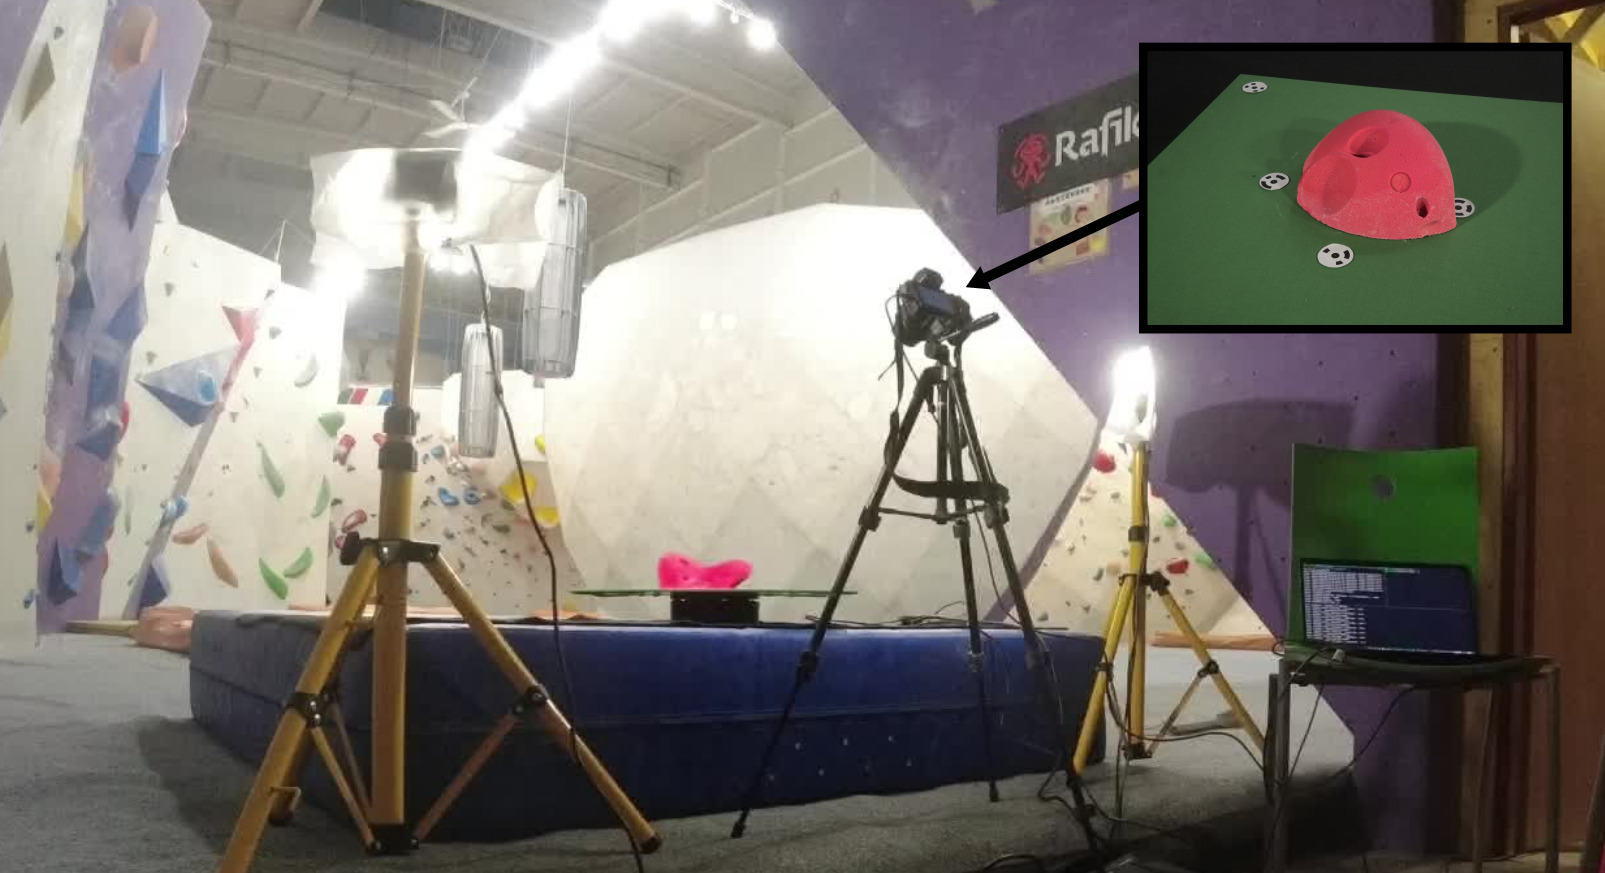
\includegraphics[width=\columnwidth]{images/setup/setup.png}
	\caption{An image of the setup during scanning, including the taken image. f-stop: 22, focal length: 38mm, ISO: 320, exposure time: 1s.}
	  
	\label{fig:setup}
\end{figure}

\subsection{Dual texture holds}
Glossy surfaces are one of the most problematic types surfaces for photogrammetry, since the angle under which they are imaged change their appearance due to light reflecting into the camera.
This poses a problem for „dual-texture“ holds which, as the name suggests, contain two textures -- a mate texture that is meant for the climber to hold (or step) onto, and the glossy texture which is usually not.
They are increasingly used in modern bouldering and sports climbing, because they give setters more freedom in creating difficult routes.

A standard way of dealing with glossy surfaces is to cover them in something that is mate.
While this does solve the problem of model generation, it ruins the texture, because the mate solution is usually opaque (and possibly requiring another set of images for texturing).

In our case, however, the solution is rather obvious -- cover them in climbing chalk (figure \ref{fig:chalk}).
Since it is mate, it reduces the reflections of the glossy surface and provides additional feature points, making it easier for the photogrammetry software to reconstruct the model.
Additionally, since climbing chalk will be applied to the holds by climber during regular usage anyway, there is no need to obtain more images for texturing.

\begin{figure}[H]
	\centering
	\subfloat{{\includegraphics[height=2.5cm]{images/holds/1.png} }}%
	\hfill
	\subfloat{{\includegraphics[height=2.5cm]{images/holds/2.png} }}%
	\hfill
	\subfloat{{\includegraphics[height=2.5cm]{images/holds/3.png} }}%
	\caption{Example of holds with chalk applied. Some reflections are still visible, but they are not as pronounced as with no chalk applied.}%
	\label{fig:chalk}
\end{figure}

\section{Editor implementation}
The editor has been created using the Unity editor, with the majority of the codebase being written in C\#.
While other options exist, such as Unreal Engine and Godot, Unity was chosen due to the author's experience with developing games using it, along with the large ecosystem of packages that could be used to simplify the implementation and allow for rapid prototyping.

Using this ecosystem, a number of freely available packages were used (with minor modifications), namely

\begin{itemize}
	\item \textbf{Quick Outline} \footnote{\url{https://assetstore.unity.com/packages/tools/particles-effects/quick-outline-115488}} -- object outline creator (for hold highlights),
	\item \textbf{OBJImport} \footnote{\url{https://assetstore.unity.com/packages/tools/modeling/runtime-obj-importer-49547}} -- an \verb|.obj| file importer (including texture files) and
	\item \textbf{StandaloneFileBrowser} \footnote{\url{https://github.com/gkngkc/UnityStandaloneFileBrowser}} -- a cross-platform file browser.
\end{itemize}

The editor is cross-platform and can be run on Mac, Windows and Linux, with the newest builds being freely available on the project GitHub page.

\subsection{Wall and hold format}
For the editor to correctly load the scene, it expects the wall and holds to be in the \verb|obj| file format, possibly with a \verb|mtl| file and a bitmap texture.
To simplify this, the editor contains a Python script to automatically import models from Clis and generate preview images and videos for them.

Additionally, the wall can contain a \verb|yaml| metadata file for wall-specific things, namely the route grades, the names of the setters and which zone the route is located in.
This is to simplify editing route properties by selecting the right option from a dropdown, instead of having to manually type it in. Here is an example of one such file:

\begin{minted}{yaml}
Grades: ["black", "purple", "red", "salmon", "blue", "yellow"]
Setters: ["Danny", "Bert"]
Zones: ["1", "2", "3", "4", "5"]
\end{minted}

\subsection{Modes}
The editor contains three modes in which can operate, with the current mode being always displayed in the top right.
While this might seem like an implementation detail, it is arguably important for user documentation and general usage, because the user always knows which state the editor.
An obvious inspiration is the Vim text editor, which makes the mode distinction similarly apparent.
The modes are the following:

\begin{itemize}
		\item \textbf{NORMAL} -- the mode the user is usually in; hovering highlights holds, which can be either picked up or selected.
		\item \textbf{HOLDING} -- the mode in which the user is holding a specific hold and can place it or switch to the next one from the selection.
		\item \textbf{ROUTE} -- the mode in which the user modifies the selected route by adding/removing new holds or modifying route parameters.
\end{itemize}

\subsection{Hold picking}
Picking which holds to place on the wall quickly is crucial for effective virtual route setting, because it dictates the time the route setting takes.
The editor contains a hold picking menu from which a subset of holds can be selected and cycled while editing.
Filtering holds can be done by selecting a specific hold color, type, manufacturer, or custom hold label.
Additionally, hovering on each of the holds rotates them around, which is useful when the static hold image isn't descriptive enough.

TODO: obrázek toho vybírání


\subsection{Import and Export}
The import and export format for the project files is a human-readable \verb|yaml| file containing information about the state of the holds, routes, paths to the models and other metadata.
This makes it easy to be used in other applications (both for viewing and modification), since it is well readable and parseable.
Here is how the format looks like:

\begin{minted}{yaml}
Player:
  Light: false # whether the player's light is on
  Position: # the player position as a vector
    x: 4.66010237
    y: 1.93126345
    z: -8.63198185
  Orientation: # the player orientation as a quaternion
    w: 0.825024903
    x: 0.117302731
    y: -0.54728353
    z: 0.0778122842

# path to the wall and the holds
WallModelPath: /home/xiaoxiae/Downloads/Wall/wall.obj
HoldModelsPath: /home/xiaoxiae/Downloads/Holds

Holds:
  f21cde933ad9: # a unique ID for the hold instance
    BlueprintId: 4bdff2704462 # an ID of the hold model
    State:
      Position: # the position of the hold in space
        x: 1.20504105
        y: 0.378549755
        z: -7.67928696
    Normal: # the normal of the wall (where is it facing)
        x: 0.994500279
        y: 0.0156783238
        z: 0.103554823
      Rotation: 0 # the hold rotation about the normal
  0436ff53a1d8:
    BlueprintId: 4bdff2704462
    State:
      Position:
        x: 1.46525836
        y: 0.472094655
        z: -8.19389153
      Normal:
        x: 0.752805889
        y: -0.0226488542
        z: 0.657852829
      Rotation: 1.21387374

Routes:
- Name: A very nice route
  Grade: blue
  Zone: 3
  Setter: Danny
  HoldIDs: # which holds the route contains
  - 0436ff53a1d8
  - f21cde933ad9

# a general list of starting and ending holds
StartingHoldIDs: ["f21cde933ad9"]
EndingHoldIDs: ["0436ff53a1d8"]

# the positions of lights around the wall + their parameters
Lights:
  Positions: []
  Intensity: 0.2 # how strong the light is
  ShadowStrength: 0.2 # how hard the shadows are
\end{minted}

\subsection{Capturing images}
The editor contains functionality for capturing the current image of the wall.
This can be done anywhere in the editor by either selecting the option from the toolbar, or by pressing \verb|Ctrl+P|.
The image is then saved to the default system „Pictures“ folder, unless configured otherwise in the settings.

TODO: some images!
